% Beamer slides (~10 min). On Overleaf: Menu -> Main document -> slides.tex, compiler pdfLaTeX.
\documentclass[aspectratio=169,11pt]{beamer}
\usetheme{default}
\usecolortheme{dove}
\setbeamertemplate{navigation symbols}{}
\setbeamertemplate{footline}[frame number]
\usepackage{booktabs,amsmath,tikz}
\usetikzlibrary{positioning,arrows.meta}
\graphicspath{{figures/}}
\definecolor{acc}{HTML}{2A78D6}
\setbeamercolor{frametitle}{fg=acc}
\setbeamercolor{title}{fg=acc}
\newcommand{\STOP}{\textsc{stop}}
\newcommand{\CONT}{\textsc{continue}}

\providecommand{\citep}[1]{}  % findings.tex cites; slides don't
\providecommand{\todo}[1]{\textcolor{red}{[TODO: #1]}}
\newcommand{\numCqwen}{0.40}
\newcommand{\tDraftQwen}{10.7}
\newcommand{\tTargetQwen}{26.5}
\newcommand{\numCsmol}{0.25}
\newcommand{\tDraftSmol}{6.6}
\newcommand{\tTargetSmol}{26.7}
  % measured values, written by `uv run python -m specrl.report_tables`
% One-paragraph findings shared by main.tex (report) and slides.tex. Numbers from results/*.csv (10 Nov 2026).

% ---- report ----
\newcommand{\resultsParagraph}{%
All four RL agents beat every baseline on both model pairs, in the simulator and in real wall-clock time.
On the RTX~3050, Value Iteration is fastest: 1.51$\times$ the target alone for Qwen and 1.75$\times$ for
SmolLM2, against 1.42$\times$ and 1.65$\times$ for the best baseline (HuggingFace's 0.4 confidence threshold)
and 1.38$\times$ and 1.57$\times$ for the best fixed draft length. REINFORCE (1.50$\times$ / 1.70$\times$) and DQN
(1.47$\times$ / 1.70$\times$) follow closely; Q-learning is last among the agents (1.47$\times$ / 1.67$\times$) but
still ahead of all baselines. The agents gain \emph{fewer} tokens per target call than the threshold rule yet
are faster: they stop earlier when a rejection is likely and so waste fewer draft steps. Speedups are larger
for SmolLM2, whose draft step is cheaper relative to its target ($c=0.25$ vs $0.40$).}

\newcommand{\heatmapSentence}{%
Value Iteration learned a clean threshold on $q$: it stops whenever the estimated chance that all drafts
survive falls below about 0.7, and continues otherwise. This is the shape SpecDec++~\citep{huang2024specdecpp}
proves optimal, and the agent was not told it: it came out of the Bellman equation. DQN and REINFORCE learned
soft thresholds around $q\approx0.3$--$0.5$; within one cell they sometimes stop and sometimes continue,
because they also read the latest token's confidence $p$ and the entropy $H$, which $q$ does not capture.
Q-learning shows the same idea, but noisily.}

\newcommand{\taskSentence}{%
The agents draft about twice as long on code and maths as on chat (Value Iteration: 2.0 tokens per round on
chat, 4.0--4.2 on code and maths) without being told the task: they read it from the draft's confidence.
Code and maths answers are formulaic (the draft matches the target 92--93\% of the time), chat is open-ended
(78\%). The largest live speedups are on code: 1.61$\times$ for Qwen and 2.03$\times$ for SmolLM2 with Value
Iteration.}

\newcommand{\lambdaSentence}{%
A cheap target call (low $\lambda$) makes the agent draft long rounds and waste rejected drafts; an expensive
one makes it stop early, and at 1.4 times the tuned value it collapses to stopping after a single token, the
failure mode anticipated in our proposal. The best speedup lies exactly at the $\lambda$ chosen by the
Dinkelbach update, which confirms the method.}

\newcommand{\simLiveSentence}{%
The simulator ranks the methods in the same order as the live benchmark (Spearman rank correlation 1.00 for
Qwen, 0.94 for SmolLM2, where DQN and REINFORCE, 0.005$\times$ apart, swap places). Live speedups are 8\%
(Qwen) and 14\% (SmolLM2) lower than simulated, because the simulator does not count the per-step cost of
computing features, querying the policy and Python control flow; that fixed overhead weighs more when the
draft step itself is cheaper (SmolLM2). Training in the simulator is therefore a reliable way to compare and
choose policies, but its absolute speedups are optimistic.}

\newcommand{\hypothesesParagraph}{%
\begin{enumerate}
  \item \emph{All four agents match or beat the best fixed-$k$ baseline}: confirmed, live and simulated, on both pairs.
  \item \emph{Value Iteration is the strongest tabular method and Q-learning approaches it}: confirmed; Value
  Iteration was the strongest method overall.
  \item \emph{DQN and REINFORCE gain from the richer state, with REINFORCE noisier}: partly. Both beat
  Q-learning but not Value Iteration, and with per-round episodes REINFORCE was not noisier.
  \item \emph{The learned policies look like a threshold on $q$}: confirmed (Figure~\ref{fig:heatmap}).
  \item \emph{Speedups are larger on the SmolLM2 pair}: confirmed (1.75$\times$ vs 1.51$\times$ live).
\end{enumerate}}

\newcommand{\seedSentence}{%
Retraining Q-learning, DQN and REINFORCE with three seeds each (Table~\ref{tab:seeds}) confirms the ranking where
the gaps are large: Q-learning is last on both pairs for every seed, and on Qwen the order Value Iteration $>$
REINFORCE $>$ DQN holds for every seed. On SmolLM2, Value Iteration, DQN and REINFORCE lie within each other's
seed ranges (2.01--2.02$\times$), so their differences there are noise.}

\newcommand{\conclusionParagraph}{%
All four algorithms learned useful stopping rules from a simulator built in minutes, and all of them beat
fixed draft lengths and HuggingFace's confidence threshold in real wall-clock time: up to 1.51$\times$
(Qwen) and 1.75$\times$ (SmolLM2) faster than the target model alone, with the same output. Model-based Value
Iteration, the simplest method, was the strongest: with an accurate model of the environment available,
planning beat learning from samples. The agents rediscovered the threshold rule that theory predicts, and
learned on their own to draft longer on predictable code and maths than on open-ended chat.}

% ---- slides ----
\newcommand{\resultsSentence}{All four agents beat every baseline live. Best: Value Iteration, 1.51$\times$
(Qwen) and 1.75$\times$ (SmolLM2) vs 1.42$\times$ / 1.65$\times$ for HuggingFace's threshold rule.}
\newcommand{\heatmapShort}{Value Iteration learned a clean threshold: \STOP{} when $q<0.7$. Nobody told it;
it is the rule SpecDec++ proves optimal. DQN and REINFORCE learned soft versions of it.}
\newcommand{\taskShort}{Agents draft about twice as long on code and maths as on chat, learned from the
draft's confidence alone. Largest live gain: code, 2.03$\times$ (SmolLM2).}
           % one-sentence findings shared by report and slides (written by hand)

\title{Learning When to Stop Drafting}
\subtitle{Reinforcement Learning for Adaptive Speculative Decoding in LLMs}
\author{Shikhar Saxena \and Vaibhav Sundriyal \and Angad Shukla}
\institute{Thapar Institute of Engineering and Technology, Patiala}
\date{November 2026}

\begin{document}

\begin{frame}
  \titlepage
\end{frame}

\begin{frame}{1. Live race}
  \centering
  \Large Demo: target alone vs target + RL agent, same prompt\\[1em]
  \normalsize \texttt{uv run python -m specrl.app}\\[1em]
  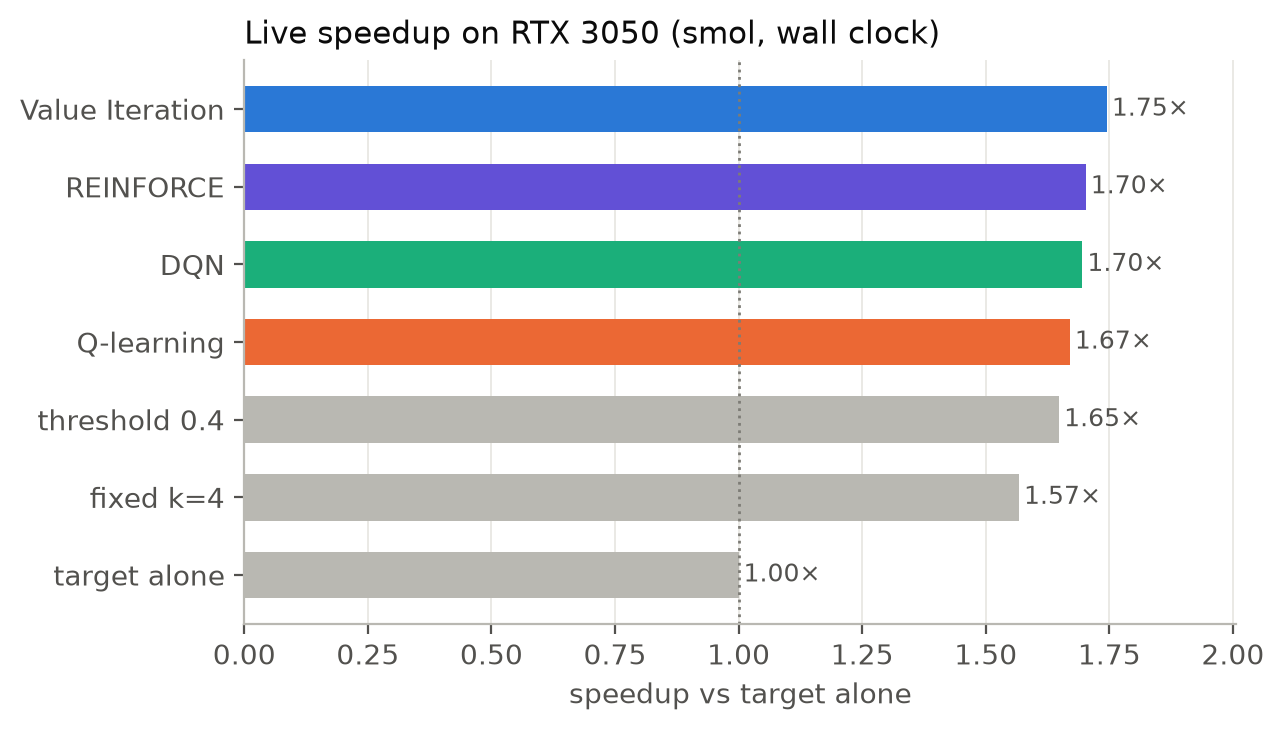
\includegraphics[height=0.55\textheight]{speedup_live_smol}
\end{frame}

\begin{frame}{2. The idea: a junior writer and a senior editor}
  \begin{itemize}
    \item \textbf{Junior writer} (small draft model) quickly drafts a few words.
    \item \textbf{Senior editor} (big target model) checks the whole draft in \emph{one} read.
    \item Too little drafting: the editor is interrupted constantly.
    \item Too much: most of the draft is crossed out.
    \item \textbf{Our RL agent is the manager} deciding, word by word, when to hand the draft over.
  \end{itemize}
  \vspace{0.5em}
  Output is \textbf{exactly} the big model's output, just faster.
\end{frame}

\begin{frame}{3. Speculative decoding in one picture}
  \centering
  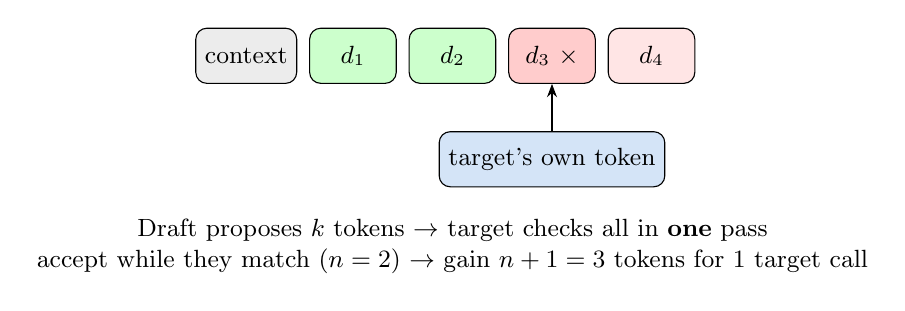
\begin{tikzpicture}[tok/.style={draw,rounded corners,minimum width=1.1cm,minimum height=0.7cm,font=\small}]
    \node[tok,fill=gray!15] (c) {context};
    \node[tok,fill=green!20,right=0.15 of c] (d1) {$d_1$ \checkmark};
    \node[tok,fill=green!20,right=0.15 of d1] (d2) {$d_2$ \checkmark};
    \node[tok,fill=red!20,right=0.15 of d2] (d3) {$d_3$ $\times$};
    \node[tok,fill=red!10,right=0.15 of d3] (d4) {$d_4$};
    \node[tok,fill=acc!20,below=0.6 of d3] (t) {target's own token};
    \draw[-{Stealth}] (t) -- (d3);
    \node[below=1.6 of d2,align=center,font=\small] {Draft proposes $k$ tokens $\to$ target checks all in \textbf{one} pass\\
      accept while they match ($n=2$) $\to$ gain $n+1 = 3$ tokens for 1 target call};
  \end{tikzpicture}
\end{frame}

\begin{frame}{4. The MDP}
  \small
  \begin{tabular}{@{}ll@{}}
    \toprule
    State & $s$ drafted so far, $p$ draft confidence, $H$ entropy,\\
          & $q=\prod p$ (chance all drafts survive), $a$ recent acceptance rate\\
    Actions & \CONT{} (draft one more) or \STOP{} (verify); forced \STOP{} at $s=8$\\
    Reward & 0 on \CONT{};\quad on \STOP{}: $r = (\min(s,n)+1) - \lambda(1+s\,c)$\\
    $c$ & $t_\text{draft}/t_\text{target}$, measured on our GPU (\numCqwen{} Qwen, \numCsmol{} SmolLM2)\\
    $\lambda$ & price of a target call; Dinkelbach: $\max \frac{\text{tokens}}{\text{time}} \Leftrightarrow \max(\text{tokens}-\lambda\,\text{time})$\\
    \bottomrule
  \end{tabular}
  \begin{align*}
    Q^*(s,\STOP) &= \mathbb{E}[\min(s,n)+1] - \lambda(1+s\,c)\\
    Q^*(s,\CONT) &= \mathbb{E}\big[\max_{a'} Q^*(s',a')\big]
  \end{align*}
\end{frame}

\begin{frame}{5. Four algorithms, one task}
  \small
  \begin{tabular}{@{}llll@{}}
    \toprule
    Algorithm & Course topic & State & Learns from \\
    \midrule
    Value Iteration & DP, Bellman & 80 table states $(s,q)$ & model counted from logs \\
    Q-learning & TD learning & 80 table states & simulated experience \\
    DQN & Deep RL & 5 features, MLP 64--64 & replay buffer + target net \\
    REINFORCE & Policy gradient & 5 features, MLP 64 & Monte Carlo returns \\
    \bottomrule
  \end{tabular}
  \vspace{1em}

  Trained in a \textbf{simulator} built from one logging pass on the GPU (2 forward passes per prompt):
  any policy can be replayed on the CPU in seconds.
\end{frame}

\begin{frame}{6. Results}
  \centering
  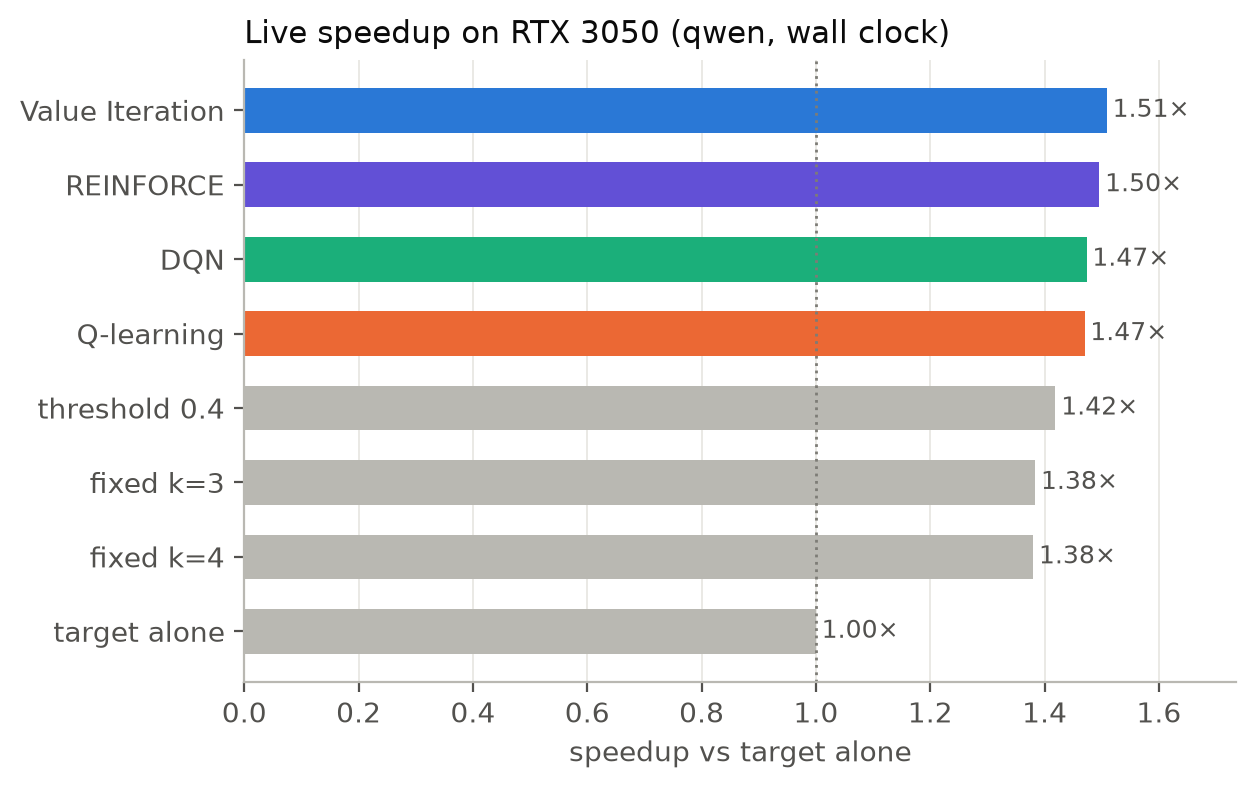
\includegraphics[height=0.42\textheight]{speedup_live_qwen}\hfill
  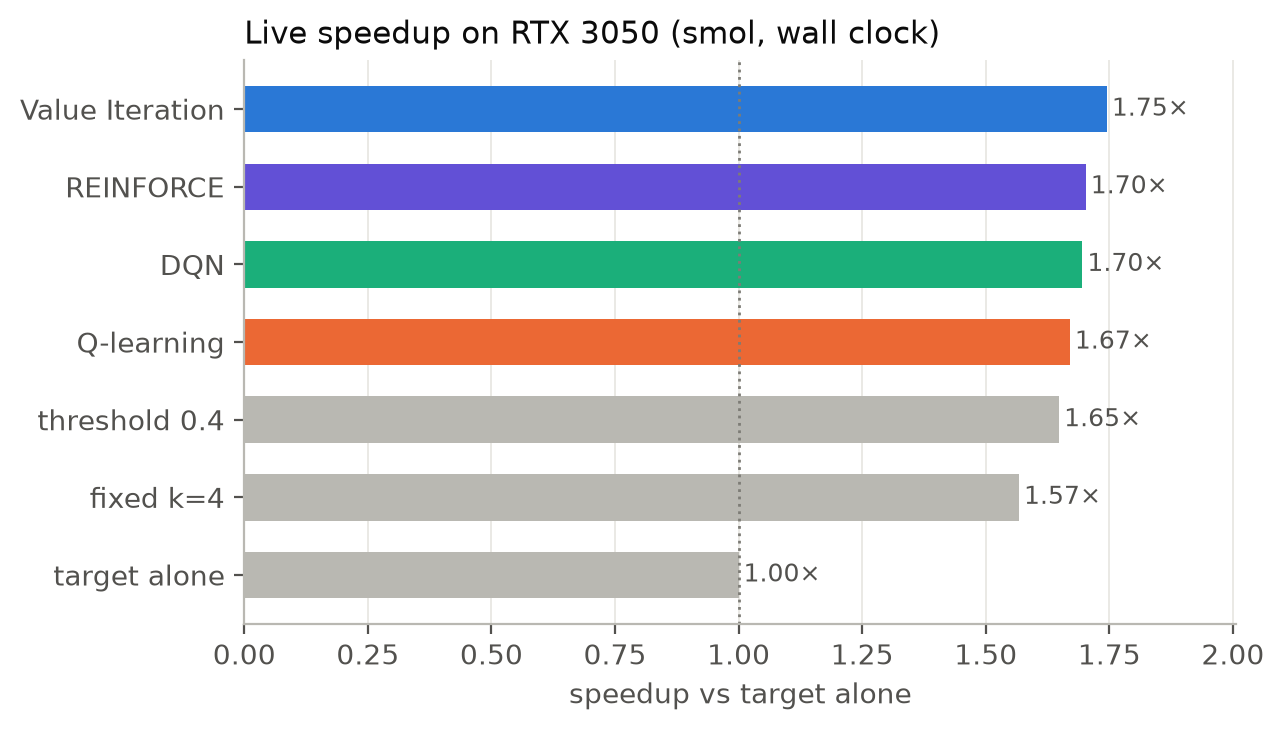
\includegraphics[height=0.42\textheight]{speedup_live_smol}\\[0.5em]
  \small \resultsSentence
\end{frame}

\begin{frame}{7. What the agent learned}
  \centering
  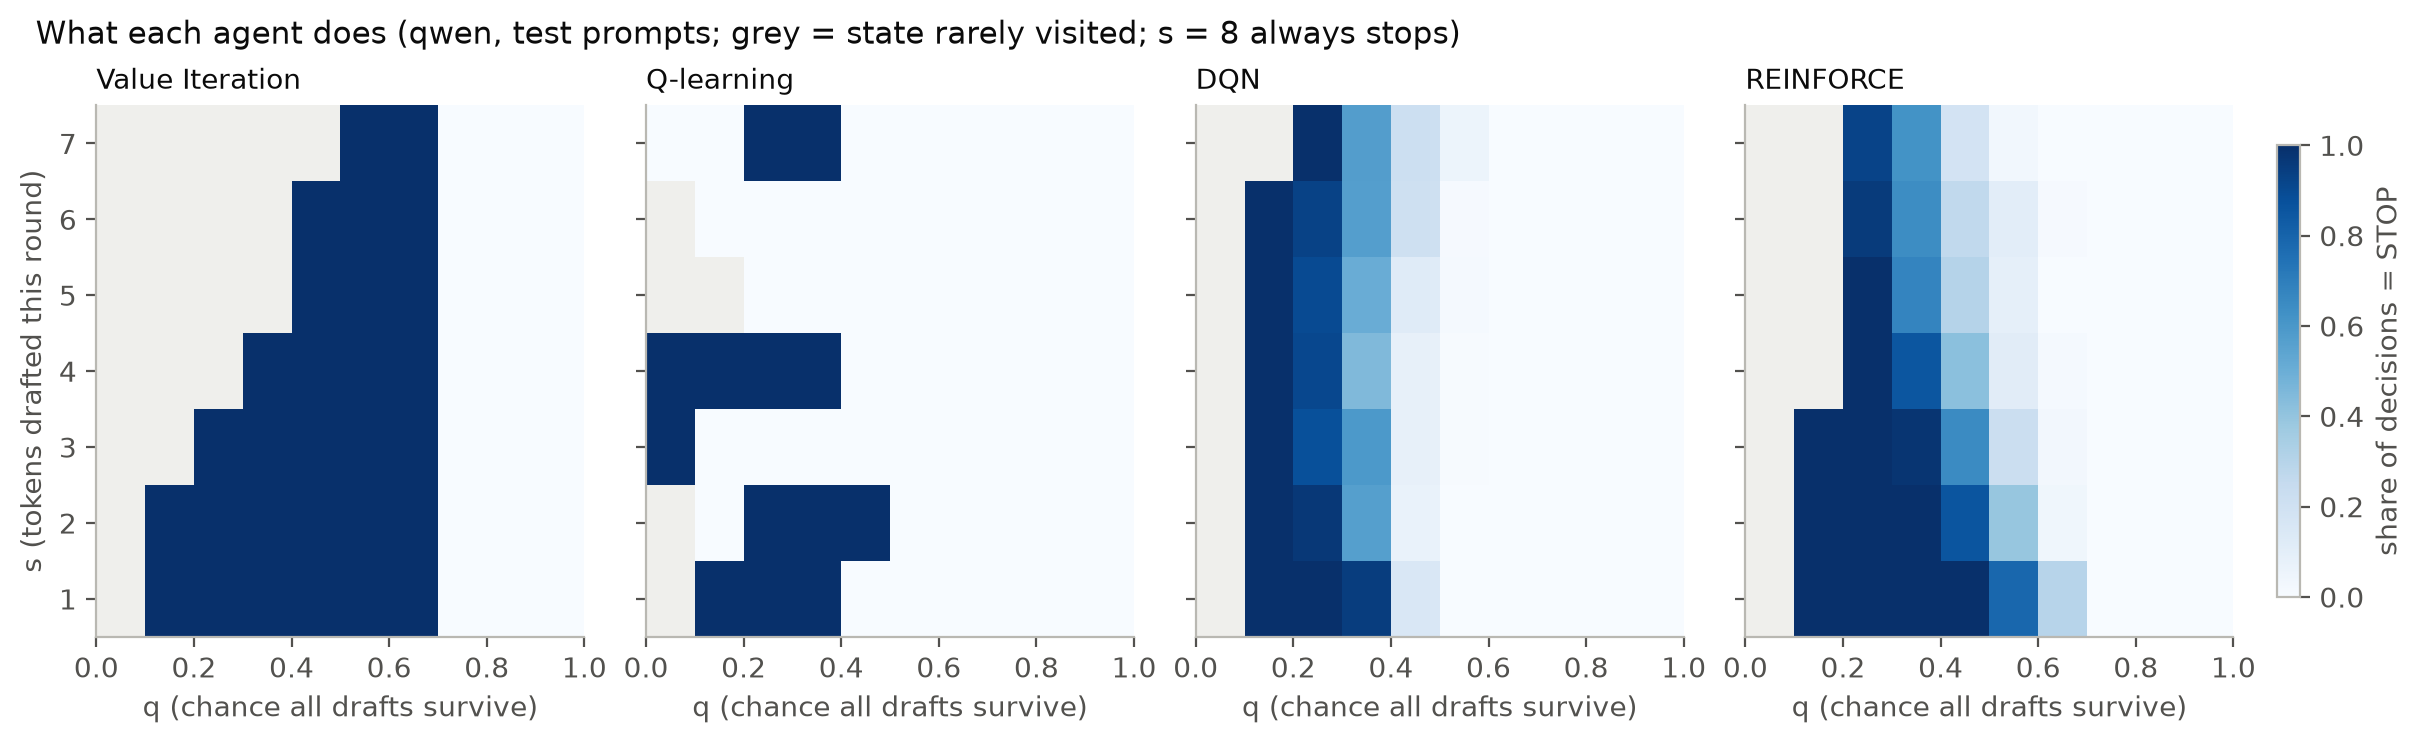
\includegraphics[width=\textwidth]{policy_heatmap_qwen}\\
  \small \heatmapShort
\end{frame}

\begin{frame}{7b. Training and per-task behaviour}
  \centering
  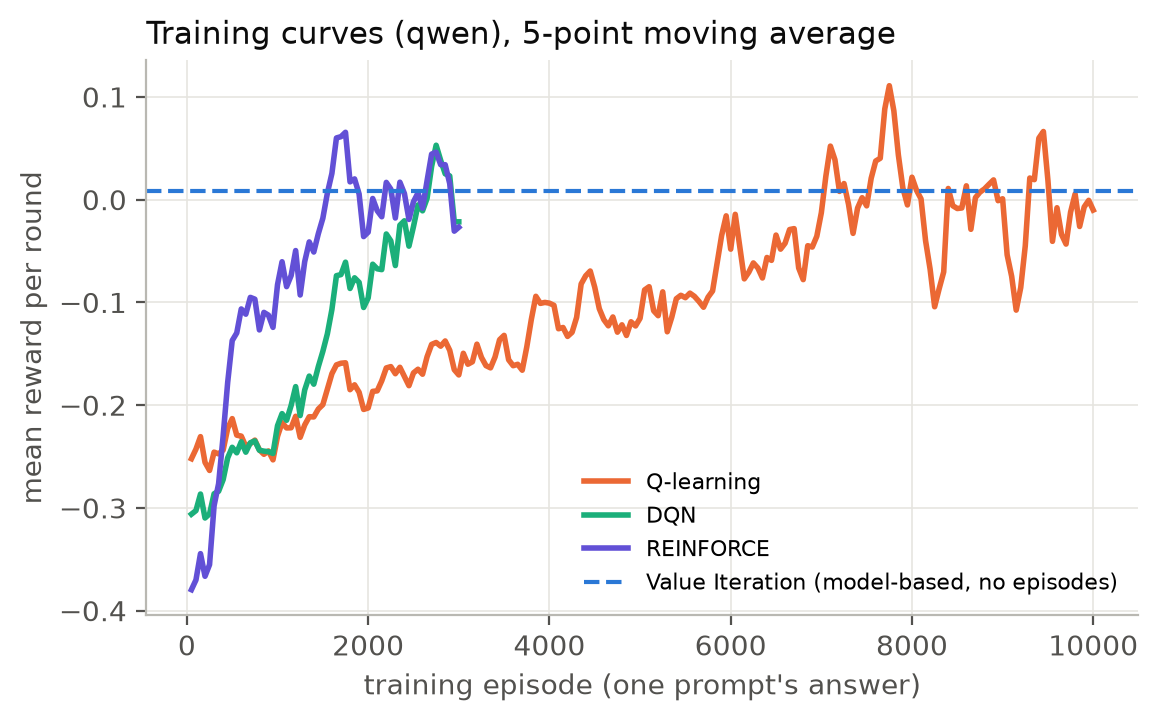
\includegraphics[height=0.45\textheight]{training_curves_qwen}\hfill
  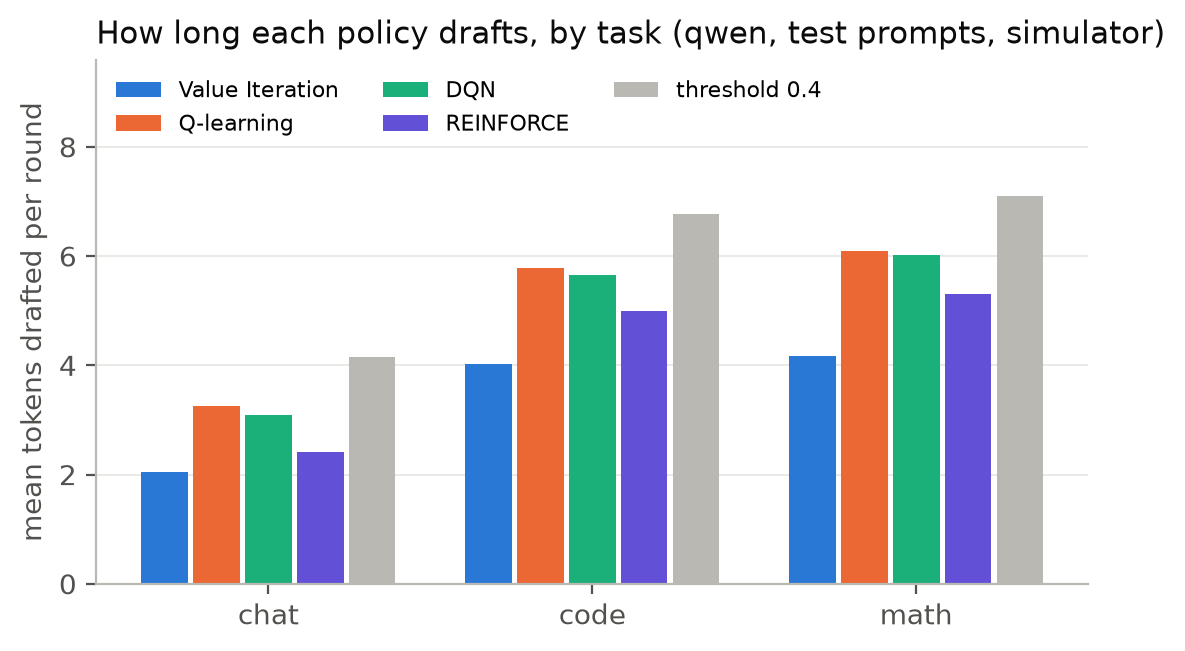
\includegraphics[height=0.45\textheight]{per_task_draft_len_qwen}\\
  \small \taskShort
\end{frame}

\begin{frame}{8. Your turn}
  \centering
  \Large Type a prompt — we race it live.\\[1.5em]
  
ormalsize Code, results, report and the full decision log are in our project repository.
\end{frame}

\end{document}
